\chapter{Logkorrelation in Cloud-Umgebungen}\label{02_jcorrelat}
\thispagestyle{fancy}

Im folgenden Abschnitt wird eine Forschungsarbeit der Fachhochschule Fulda 
\cite{reissmann} vorgestellt. Ziel der Forschung war und ist es, ein gut skalierendes 
System zu entwickeln um eine automatisierte Auswertung von \textit{Syslog}-Meldungen in 
Cloud-Umgebungen bereit zu stellen. Aufgrund der enormen Datenmengen die in solchen 
Umgebungen anfallen kann eine Auswertung nur mittels korrelations- und 
Aggregationsverfahren geschehen. Um dieses Ziel zu erreichen kommen verschiedene 
Standards und eine Reihe von Software-Lösungen zum Einsatz.

Nachfolgend werden einige wichtige Begriffe geklärt, die Anforderungen identifiziert, die 
verwendeten Standards und die eingesetzte Software erläutert und im Weiteren Verlauf des 
Abschnitts wird anhand eines Beispiels eine \textit{syslog}-Korrelation vorgenommen.

\section{Anforderungen}\label{anforderungen}

Viele Unternehmen haben in den letzten Jahren einen großen Teil ihrer IT-Infrastruktur 
ausgelagert. Laut Analysen werden bis 2025 80 \% aller Unternehmen \cite{web_ix} 
weltweit ihre eigene Rechenzentrumsinfrastruktur abgeschaltet haben. Die wenigen Anbieter 
von Cloud-Infrastruktur stehen in Konkurrenz miteinander, daher existieren auch keine 
einheitlichen Schnittstellen um auf die Cloud-Konfigurationen zuzugreifen. Für die 
Überwachung, speziell von Sicherheitskritischen Ereignissen, stehen ebenso nur 
proprietäre Schnittstellen jedes Anbieters zur Verfügung. Aus diesem Grund soll ein 
System geschaffen werden, das die gewaltige Menge an aufkommenden Logdaten, unabhängig 
vom Anbieter, analysiert und sicherheitskritische Ereignisse unverzüglich zu 
identifiziert. Insbesondere soll das System das dynamisch sinkende und wachsende 
\textit{syslog}-Aufkommen beherrschen können. Denn durch die fluide Kostenstruktur der 
Cloud-Anbieter können schnell neue virtuelle Maschinen erstellt und entfernt werden, je 
nachdem wie viel Leistung der Kunde gerade benötigt.
Darüber hinaus sollen Meldungen auch persistent gespeichert werden, vornehmlich zur 
Erstellung von Trends und Langzeitanalysen, dabei soll der benötigte Speicherplatz so 
gering wie möglich gehalten werden.

\section{Beispielszenario}\label{szenario}

Im weiteren Verlauf dieses Kapitels soll zur detaillierteren Darstellung der 
Leistungsfähigkeit einer automatischen \textit{syslog}-Korrelation ein gängiges 
Angriffsszenario dienen. Eine \textit{ssh}-BruteForce Attacke auf eine beliebige Anzahl
an überwachten Systemen. Dabei soll genau der eine erfolgreiche Login innerhalb  der 
enormen Anzahl an erfolglosen oder ungültigen Versuchen identifiziert werden. Dieses 
recht einfache Szenario ist bei der erheblichen Anzahl an möglichen Systemen (10K+) 
manuell unmöglich zu bewerkstelligen.

\newpage
\section{JCorrelat}\label{sec_jcorrelat}

In Abbildung \ref{pic:jcorrelat} \cite[47]{reissmann} ist der schematische Aufbau von 
JCorrelat dargestellt, ein Prototyp der die Anforderungen aus Abschnitt 
\ref{anforderungen} erfüllen soll. Die hinzugefügten Nummern dienen der Übersichtlichkeit 
im weiteren Erklärungsverlauf.   

\begin{figure}[htbp]
    \caption{Aufbau von JCorrelat}
    \label{pic:jcorrelat}\vspace{0.2cm}
    \centering
    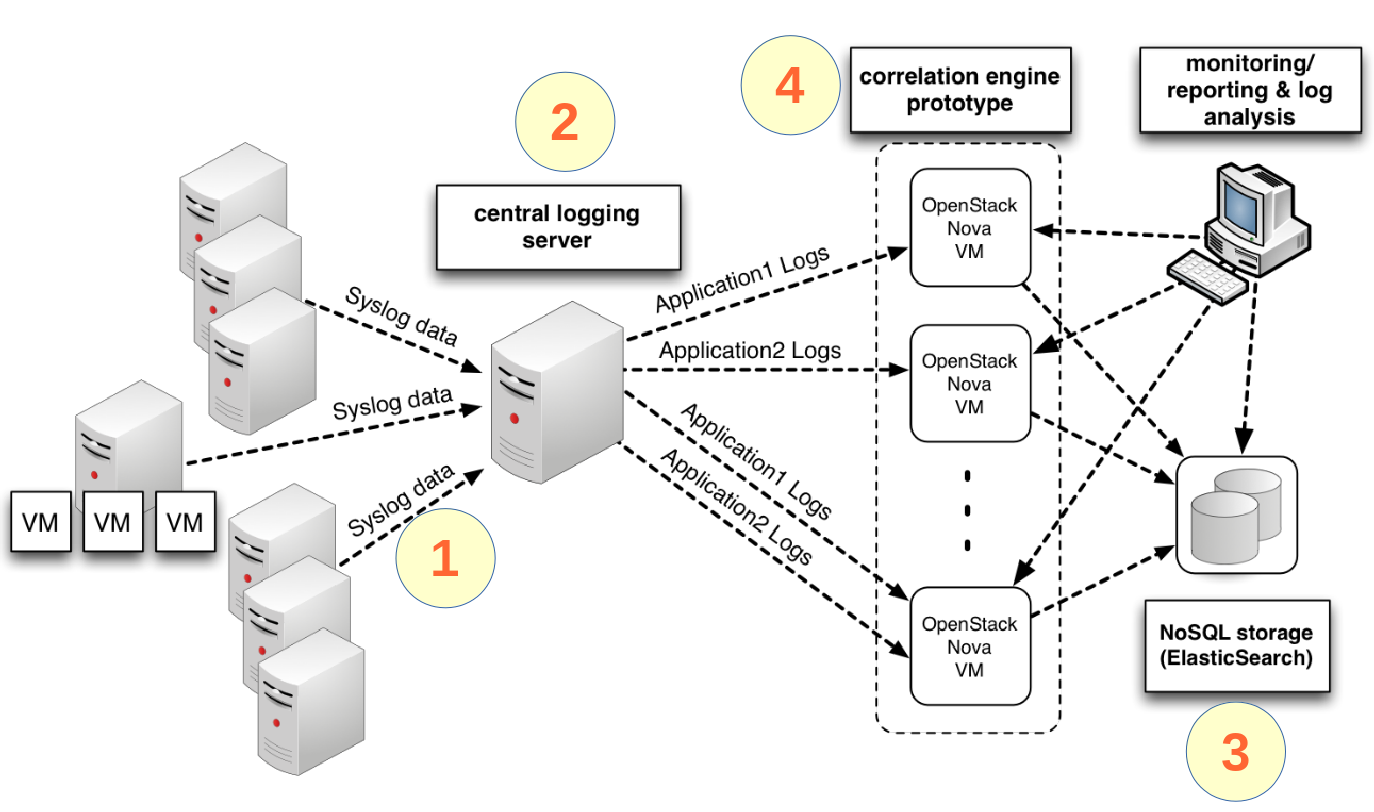
\includegraphics[scale=0.36]{img/schema-correlat}
    
\end{figure}

\subsection{Syslog-Protokoll} \label{syslog-proto}




\subsection{Konsolidierung von Syslog-Meldungen}\label{syslog-konsolidierung}
\subsection{persistente Speicherung}\label{nosql}
\subsection{Korrelation von Syslog-Meldungen}\label{syslog-korrelation}